\documentclass[11pt]{article}
\usepackage[sc]{mathpazo}
\usepackage{amsmath,pifont}
\usepackage{fullpage}
\usepackage[authoryear,sectionbib,sort]{natbib}
\linespread{1.7}
\usepackage[utf8]{inputenc}
\usepackage{lineno}

\usepackage{graphicx} 
\usepackage{tabularx,setspace}

\title{Density-dependent selection in evolutionary genetics: a lottery model of Grime's triangle}
%\author{Jason Bertram $^{1,\ast}$ \\ 
%Joanna Masel $^{1}$}

\date{}

\begin{document}

\maketitle

%\noindent{}1. Department of Ecology and Evolutionary Biology, University of Arizona, Tucson, AZ 85721.

%\noindent{}$\ast$ Corresponding author; e-mail: jbertram@email.arizona.edu.


\bigskip

\textit{Manuscript elements}: 

\bigskip

\textit{Keywords}: r/K selection, absolute fitness, eco-evo, interference competition, competition-colonization trade-off.

\bigskip

\textit{Manuscript type}: Article. 
% Or e-article, note, e-note, natural history miscellany,
% e-natural history miscellany, comment, reply, symposium, or
% countdown to 150.

\bigskip

\noindent{\footnotesize Prepared using the suggested \LaTeX{} 
template for \textit{Am.\ Nat.}}

\linenumbers{}
\modulolinenumbers[3]

\newpage{}

\section*{Abstract}

Fitness is typically represented in heavily simplified terms in evolutionary genetics, often using constant selection coefficients. This excludes fundamental ecological factors such as dynamic population size or density-dependence from the most genetically-realistic treatments of evolution, a problem that inspired MacArthur's influential but problematic $r$/$K$ theory. Following in the spirit of $r$/$K$-selection as a general-purpose theory of density-dependent selection, but grounding ourselves empirically in ``primary strategy'' trait classification schemes like Grime's triangle, we develop a new model of density-dependent selection which revolves around territorial contests. To do so, we generalize the classic lottery model of territorial acquisition, which has primarily been used for studying species co-existence questions, to accommodate arbitrary densities. We use this density-dependent lottery model to predict the direction of trait evolution under different environmental conditions and thereby provide a mathematical underpinning for Grime's verbal scheme. We revisit previous concepts of density-dependent selection, including $r$ and $K$ selection, and argue that our model distinguishes between different aspects of fitness in a more natural and intuitive manner.

\newpage{}


``...the concept of fitness is probably too complex to allow of a useful mathematical development. Since it enters fundamentally into many population genetics considerations, it is remarkable how little attention has been paid to it.'' --- Warren J. Ewens, Mathematical Population Genetics I, 2004 

Evolutionary models differ greatly in their treatment of fitness. In models of genetic evolution, genotypes are typically assigned constant (or frequency-dependent) selection coefficients describing the change in their relative frequencies over time. This simplified treatment of selection facilitates genetic realism, and can be justified over sufficiently short time intervals \citep[p. 276]{ewens_2004}. The emphasis here is to infer past selection, migration and demographic change given a sample of nucleotide sequences, or to predict how allele frequencies change over time based on their fitness effects, population structure, genetic drift and linkage. The resulting picture of evolution excludes basic elements of the ecological underpinnings of selection, including density dependence, and how selection affects population size. This complicates the inference of past selection, because demographic changes can look geneaologically very similar to selective frequency changes \citep{barton_1998}. 

%Separately fitting demographic models to data on ostensibly neutral sites, and then inferring selection against this demographic background, has had mixed success due to linkage \citep{schrider_2016}.

By contrast, models of phenotypic trait evolution use absolute fitness functions to describe how some traits of interest affect survival and reproduction in particular ecological scenarios \citep{metz_1992,diekmann_2004}. These fitness functions can be quite problem-specific and often only account for a few traits at a time. The emphasis here is on the conditions for invasion from low frequencies and co-existence, rather than frequency or abundance trajectories over time. For instance, adaptive dynamics uses ``invasion fitness'' to explore the consequences of eco-evolutionary feedbacks \citep{diekmann_2004}.

It is challenging to generalize beyond particular traits or ecological scenarios to model fundamentally different forms of selection. Perhaps this is not surprising given that fitness is such a complex quantity, dependent on all of a phenotype's functional traits \citep{violle_2007} and its environment. A detailed, trait-based, predictive model of fitness would be enormously complicated and situation-specific. It is therefore easy to doubt the feasibility of a simplified, general mathematical treatment of fitness \citep[p. 276]{ewens_2004}. For example, MacArthur's famous $r$/$K$ scheme \citep{macarthur_1962,macarthur_1967} is now almost exclusively known as a framework for understanding life-history traits, and judged on its failure in that role \citep{pianka_1970,stearns_1977,boyce_1984,reznick_2002}. However, the r/K scheme's original purpose was to extend the existing population-genetic treatment of selection to account for population density \citep{macarthur_1962}. Few attempts have been made to develop it further along these lines. 

Empirical trait classification studies have suggested the existence of a few ``primary strategies'', reflecting broadly distinct responses to selection \citep{winemiller_2015}. Grime famously considered \citep{grime_1974,grime_1977,grime_1988,westoby_1998} two broad determinants of population density: stress (persistent hardship e.g. due to resource scarcity or unfavorable temperatures) and disturbance (intermittent destruction of vegetation e.g. due to trampling, herbivory, pathogens, extreme weather or fire).  The extremes of these two factors define three primary strategies denoted by C/S/R respectively (Fig. \ref{fig:grimeschematic}): competitors ``C'' excel in low stress, low disturbance environments; stress tolerators ``S'' excel in high stress, low disturbance environments; and ruderals ``R''  excel in low stress, high disturbance environments. Population persistence is not possible in high-stress, high-disturbance environments. Grime showed that measures of C, S and R across a wide range of plant species are anti-correlated, so that strong C-strategists are weak S and R strategists, and so on, creating a triangular C/S/R ternary plot \citep{grime_1974}. Similar schemes were proposed for insects \citep{southwood_1977}, fishes \citep{winemiller_1992}, and zooplankton \citep{allan_76}. More recently, modern hierarchical clustering techniques have revealed distinct trait clusters in corals analogous to Grime's primary strategies \citep{darling_2012}. These empirical findings suggest that functional traits contribute to fitness predominantly via a few key factors such as intrinsic reproductive rate or stress-tolerance.

\begin{figure}
\centering
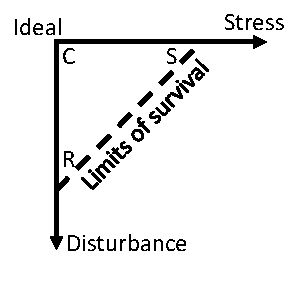
\includegraphics[scale=1]{grimeschematic.pdf}
\caption{\label{fig:grimeschematic} Schematic of Grime's triangle. The two axes show increasing levels of environmental stress and disturbance, respectively. Population persistence is not possible if the combination of stress and disturbance is too large (dashed line). This creates a triangle, each corner of which corresponds to a ``primary strategy''.} 
\end{figure}

Here we explore the interplay between some ``key factors'' of fitness in a simplified, territorial model of growth, dispersal and competition. This broadly follows the original spirit of MacArthur's $r/K$ scheme. More specifically, our aim is to begin adding some ecological realism to population genetics' time-depedendent, genetically-focused view of evolution. We revisit the classic lottery model of \cite{chesson_1981}, which has two features that make it well suited for this role, but one critical flaw that we rectify here.

The first feature is that the lottery representation of competition is  particularly concise. Mature individuals (``adults'') each require their own territory, whereas newborn individuals (``propagules'') disperse to, and subsequently compete for, territories made available by the death of adults. Territorial contest among propagules leaves a single victorious adult per territory, the victor chosen at random from the propagules present, with probabilities weighted by a coefficient for each type representing competitive ability, akin to a lottery \citep{sale_77}. By comparison, coefficients for the pairwise effects of types on each other (e.g. the $\alpha$ coefficients in the generalized Lotka-Volterra equations and the associated concept of ``$\alpha$-selection''; \citealt{gill_1974,case_1974,joshi_2001}), or  explicit resource consumption \citep{tilman_1982}, are much more complicated. The second feature is the close connection between the lottery model and one of the foundational models of population genetics, the Wright-Fisher model of genetic drift, which we discuss further below. 

The critical flaw of the classic lottery model is that it breaks down at low densities (few propagules dispersing to each territory), precluding density-dependent behaviour. Our first task is to analytically extend the classic lottery model to correctly account for low density behavior (sections ``Model'' and ``Mean field approximation'').

Using our extended lottery model, we then revisit Grime's C/S/R scheme,  and evaluate how C/S/R manifests at the level of within-population genotypic evolution (as opposed to phenotypic divergence between species; sections ``Invasion of rare genotypes and coexistence'' and ``Primary strategies and Grime's triangle''). This represents a ``sanity check'' on our density-dependent lottery model. The resulting formulation of the C/S/R scheme is mathematical, in contrast to Grime's original verbal and descriptive approach, which is a recognized hindrance to the evaluation or broader application of the C/S/R scheme (e.g. \citealt{tilman_2007}).

We then explore some time-dependent behavior of our extended lottery model. Taking an example inspired by recent studies of rapid, seasonal evolution in \textit{Drosophila} \citep{bergland_14}, we discuss how environmental fluctuations might stabilize polymorphisms in the presence of cyclical population density. 

%Fitness models like Eq. \eqref{eq:master} may help to address to these difficulties since they do not artificially separate the dynamics of abundance and frequency. 
 
\section*{Model}\label{sec:model}

We assume that reproductively mature individuals (``adults'') each require their own territory to survive and reproduce (Fig.~\ref{fig:lottery}). All territories are identical, and the total number of territories is $T$. Time $t$ advances in discrete iterations, each representing the time from birth to reproductive maturity. In iteration $t$, the number of adults of the $i$'th genotype is $n_i(t)$, the total number of adults is $N(t)=\sum_i n_i(t)$, and the number of unoccupied territories is $U(t)=T-N(t)$. 

We assume that the $n_i$ and $T$ are large enough that stochastic fluctuations in the $n_i$ (``drift'') can be ignored. We derive deterministic equations for the expected change in the $n_i$ over time, leaving the evaluation of drift for future work. In particular, we do not evaluate the initial stochastic behaviour of adaptive mutant lineages while they are at low abundance. When considering mutations, we restrict our attention to the earliest deterministic behavior of mutant lineages while they are still at low frequency (the transition to deterministic growth occurs at an abundance of order equal to their inverse expected absolute growth rate; \citealt{uecker_2011}).


\begin{figure}
\centering
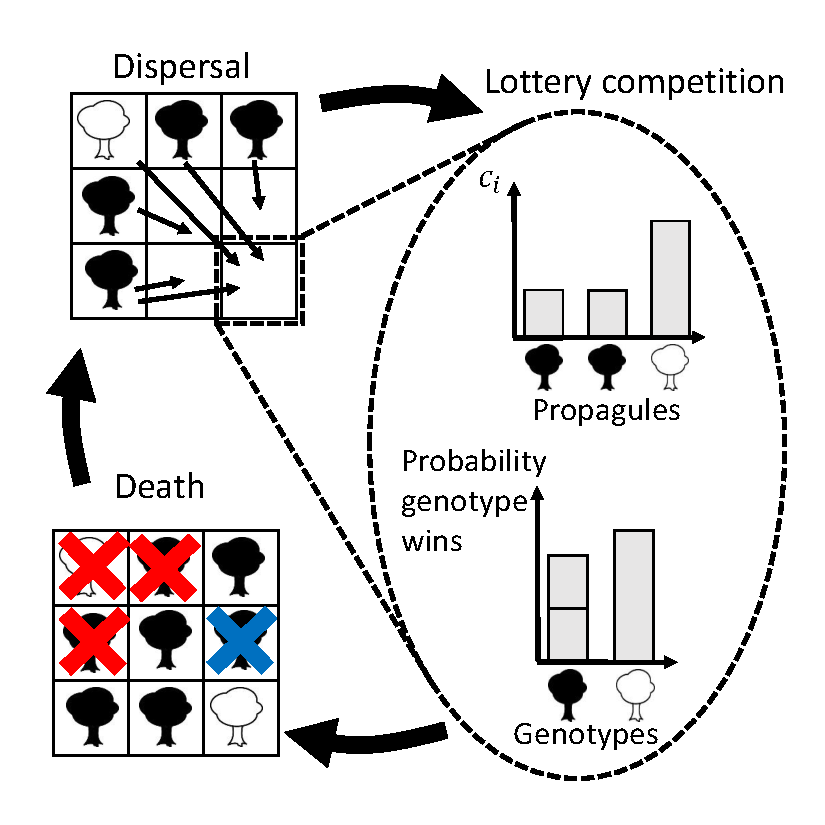
\includegraphics[scale=0.8]{lottery.pdf}
\caption{\label{fig:lottery} Each iteration of our lottery model has three main elements. First, propagules are produced by adults which are dispersed at random over the unoccupied territories (only propagules landing on unoccupied territories are shown). Lottery competition then occurs in each unoccupied territory (competition in only one territory is illustrated): each genotype has a probability proportional to $b_i n_i c_i$ of securing the territory. Then occupied territories are freed up by adult mortality. In Eq. \eqref{eq:delttot} and most of the paper, only adults can die (red crosses), but we will also consider the case where juveniles die (blue cross; section ``Primary strategies and Grime's triangle'').}
\end{figure}

Each iteration, adults produce new offspring (``propagules''), $m_i$ of which disperse to unoccupied territories. We assume that adults cannot be ousted from their territories, so that $m_i$ only includes propagules landing on unoccupied territories. Propagules disperse at random over the unoccupied territories, regardless of distance from their parents, and independently of each other. There is no interaction between propagules (e.g. avoidance of territories crowded with propagules). Loss of propagules during dispersal is subsumed into $m_i$. 

In general, $m_i$ will increase with $n_i$, and will depend on population density $N$. For example, if $b_i$ is the number of successfully dispersing propagules produced per genotype $i$ adult, then the loss of propagules due to dispersal to occupied territories implies $m_i=b_i(1-N/T)n_i$, akin to Levins' competition-colonization model \citep{levins_71,tilman_94}. In section ``Cyclical birth and death rates'' we evaluate Eq. \eqref{eq:master} numerically using this functional form for $m_i$, with $b_i$ assumed to be constant. 

In the sections ``Invasion of rare genotypes and coexistence'' and ``Primary strategies and Grime's triangle'', we assume the simpler form $m_i=b_i n_i$, with constant $b_i$, meaning that all propagules land on unoccupied territories (a form of directed dispersal). This simplifies the mathematics without affecting the results of those sections, which only depend on the low-frequency invasion behavior of Eq. \eqref{eq:master}. Note that due to our assumption of uniform dispersal, the parameter $b_i$ can be thought of as a measure of ``colonization ability'', which combines fecundity and dispersal ability \citep{levins_71,tilman_94,bolker_99}. 

The number of individuals of the $i$'th genotype landing in any particular territory is denoted $x_i$. We assume that $x_i$ follows a Poisson distribution $p_i(x_i)=l_i^{x_i} e^{-l_i}/x_i!$, where $l_i=m_i/U$ is the mean territorial propagule density. This only approximates uniform random dispersal, but is essentially exact provided that the $n_i$ are large enough that drift can be ignored (Appendix A).

When multiple propagules land on the same territory, the victor is determined by lottery competition: genotype $i$ wins a territory with probability $c_i x_i/\sum_j c_j x_j$, where $c_i$ is a constant representing relative competitive ability (Fig. \ref{fig:lottery}). 

In the classic lottery model \citep{chesson_1981}, unoccupied territories are assumed to be saturated with propagules from every genotype $l_i\gg 1$. From the law of large numbers, the composition of propagules in each territory will then not deviate appreciably from the mean composition $l_1,l_2,\ldots,l_G$ ($G$ is the number of genotypes present), and so the probability that genotype $i$ wins any particular unoccupied territory is approximately $c_i l_i/\sum_j c_j l_j$. Let $\Delta_+ n_i$ denote the number of territories won by genotype $i$. Then $\Delta_+ n_1,\Delta_+ n_2,\ldots,\Delta_+ n_G$ follow a multinomial distribution with $U$ trials and success probabilities $\frac{c_1 l_1}{\sum_j c_j l_j},\frac{c_2 l_2}{\sum_j c_j l_j},\ldots,\frac{c_G l_G}{\sum_j c_j l_j}$, respectively. Genotype $i$ is expected to win $c_i l_i/\sum_j c_j l_j$ of the $U$ available territories, and deviations from this expected outcome are small (since $T$ is large by assumption), giving 
\begin{equation}
\Delta_+ n_i(t)=\frac{c_i l_i}{\sum_j c_j l_j}U(t)=b_i n_i\frac{1}{L}\frac{c_i}{\overline{c}}, \label{eq:lottery}
\end{equation}
where $\overline{c}=\sum_j c_j m_j/M$ is the mean propagule competitive ability for a randomly selected propagule, $L=M/U$ is the total propagule density and $M=\sum_j m_j$ is the total number of propagules. 

There is a close connection between the classic lottery model and the Wright-Fisher model of genetic drift \citep{svardal_2015}. In the Wright-Fisher model, genotype abundances are sampled each generation from a multinomial distribution with success probabilities $w_i n_i/\sum_j w_j n_j$, where $w$ is relative fitness and the $n_i$ are  genotype abundances in the preceding generation. Population size $N$ remains constant. This is mathematically equivalent to the classic lottery model with non-overlapping generations ($d_i=1$ for all $i$) and $w_i=b_i c_i$. Thus, the classic lottery model allows us to replace the abstract Wright-Fisher relative fitnesses $w_i$ with more ecologically-grounded fecundity, competitive ability and mortality parameters $b_i$, $c_i$ and $d_i$, respectively. Since birth and death rates affect absolute abundances, this allows us to evaluate selection at different densities (after appropriate extensions are made), in an otherwise very similar model to the canonical Wright-Fisher. We therefore expect that drift in our extended lottery model should be similar to that in the Wright-Fisher model, but we leave this for future work. 

In our extension of the classic lottery model, we do not restrict ourselves to high propagule densities. Eq. \eqref{eq:lottery} is nonsensical at low densities ($l_i\ll 1$): genotype $i$ can win at most $m_i$ territories, yet Eq. \eqref{eq:lottery} demands $c_i l_i/\sum_j c_j l_j$ of the $U$ unoccupied territories, for any value of $U$. Intuitively, the cause of this discrepancy is that individuals are discrete. Genotypes with few propagules depend on the outcome of contests in territories where they have at least one propagule present, not some small fraction of a propagule as would be implied by small $l_i$ in the classic lottery model. In other words, deviations from the mean propagule composition $l_1,l_2,\ldots,l_G$ are important at low density. 

We expect that a fraction $p_1(x_1)\ldots p_G(x_G)$ of the $U$ unoccupied territories will have the propagule composition $x_1,\ldots,x_G$. Genotype $i$ is expected to win $c_i x_i/\sum_j c_j x_j$ of these. Ignoring fluctuations about these two expectations (due to our no-drift, large $T$, large $n_i$ approximation), genotype $i$'s territorial acquisition is given by
\begin{equation}
\Delta_+ n_i(t)=U(t)\sum_{x_1,\ldots,x_G} \frac{c_i x_i}{\sum_j c_j x_j} p_1(x_1)\ldots p_G(x_G), \label{eq:growthsumuncoupled}
\end{equation}
in our extended lottery model, where the sum only includes territories with at least one propagule present. Note that unlike the classic lottery model, not all unoccupied territories are claimed each iteration, since under Poisson dispersal a fraction $e^{-L}$ remain unoccupied.

For the majority of this manuscript we assume that mortality only occurs in adults (setting aside the juvenile deaths implicit in territorial contest), and at a constant, genotype-specific per-capita rate $d_i$, so that the overall change in genotype abundances is
\begin{equation}
\Delta n_i(t)=\Delta_+ n_i(t)-d_i n_i(t). \label{eq:delttot}
\end{equation}
This seems reasonable in the absence of disturbances; when we come to consider the effects of disturbances (Section ``Primary strategies and Grime's triangle''), we will incorporate disturbance-induced mortality in competing juveniles (Fig.~\ref{fig:lottery}).   

\section*{Results}

\subsection*{Mean Field Approximation}

Eq. \eqref{eq:growthsumuncoupled} involves an expectation over the time-dependent dispersal distributions $p_i$, and is thus too complicated to give intuition about the dynamics of density-dependent lottery competition. We now evaluate this expectation using a ``mean field'' approximation. 

Similarly to the high-$l_i$ approximation of classic lottery model, we replace the $x_i$ with appropriate mean values, although we cannot simply replace $x_i$ with $l_i$. For a genotype with low propagule density $l_i\ll 1$, we have $x_i=1$ in the territories where its propagules land, and so its growth comes entirely from territories which deviate appreciably from $l_i$. To account for this, we separate Eq. \eqref{eq:growthsumuncoupled} into $x_i=1$ and $x_i>1$ parts. Our more general mean field approximation only requires that there are no large discrepancies in competitive ability (i.e. we do not have $c_i/c_j\gg 1$ for any two genotypes). We obtain (details in Appendix B)
\begin{equation}
\Delta_+ n_i(t)\approx b_i n_i\left[e^{-L}+(R_i+A_i)\frac{c_i}{\overline{c}}\right], \label{eq:master}
\end{equation}
where
\begin{equation}
R_i=\frac{\overline{c}e^{-l_i}(1-e^{-(L-l_i)})}{c_i +\frac{L-1+e^{-L}}{1-(1+L)e^{-L}}\frac{\overline{c}L- c_il_i}{L-l_i}},\label{eq:Dr}
\end{equation}
and
\begin{equation}
A_i=\frac{\overline{c}(1-e^{-l_i})}{\frac{1-e^{-l_i}}{1-(1+l_i)e^{-l_i}}c_il_i+\frac{1}{L-l_i}\left(L\frac{1-e^{-L}}{1-(1+L)e^{-L}}-l_i\frac{1-e^{-l_i}}{1-(1+l_i)e^{-l_i}}\right)\sum_{j\neq i}c_jl_j}.\label{eq:Da}
\end{equation}

Comparing Eq. \eqref{eq:master} to Eq. \eqref{eq:lottery}, the classic lottery per-propagule success rate $c_i/\overline{c}L$ has been replaced by three separate terms. The first, $e^{-L}$, accounts for propagules which land alone on unoccupied territories; these territories are won without contest. The second, $R_i c_i/\overline{c}$ represents competitive victories when the $i$ genotype is a rare invader in a high density population: from Eq. \eqref{eq:Dr}, $R_i\rightarrow 0$ when the $i$ genotype is abundant ($l_i\gg 1$), or other genotypes are collectively rare ($L-l_i\ll 1$). The third term, $A_ic_i/\overline{c}$, represents competitive victories when the $i$ genotype is abundant: $A_i\rightarrow 0$ if $l_i\ll 1$. The relative importance of these three terms varies with both the overall propagule density $L$ and the relative propagule frequencies $m_i/M$. If $l_i\gg 1$ for all genotypes, we recover the classic lottery model (only the $A_ic_i/\overline{c}$ term remains, and $A_i\rightarrow 1/L$).  

Fig.~\ref{fig:simcomp} shows that Eq. \eqref{eq:master} (and its components) closely approximate direct simulations of random dispersal and lottery competition over a wide range of propagule densities. Two genotypes are present, one of which is at low frequency. The growth of the low-frequency genotype relies crucially on the low-density competition term $R_i c_i/\overline{c}$, and also to a lesser extent on the high density competition term $A_i c_i/\overline{c}$ if $l_1$ is large enough (Fig.~\ref{fig:simcomp}b). On the other hand, $R_i c_i/\overline{c}$ is negligible for the high-frequency genotype, which depends instead on high density territorial victories (Fig.~\ref{fig:simcomp}d). Fig. 3 also shows the breakdown of the classic lottery model at low propagule densities.

\begin{figure}
\centering
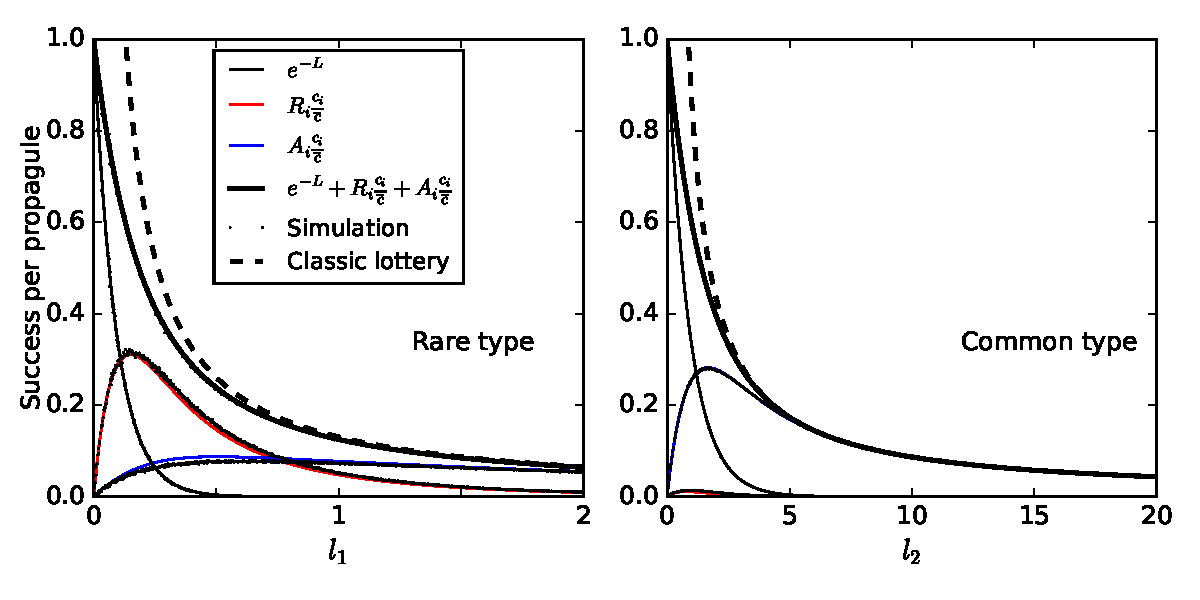
\includegraphics[scale=0.7]{simulationcomparison.pdf}
\caption{\label{fig:simcomp} The change in genotype abundances in a density dependent lottery model is closely approximated by Eq. \eqref{eq:master}. $\Delta_+ n_i/m_i$ from Eq. \eqref{eq:master} (and its separate components) are shown, along with direct simulations of random dispersal and lottery competition over one iteration over a range of propagule densities ($U$ is varied between $5\times 10^3$ and $10^6$ with $m_1=10^4$ and $m_2=9\times 10^4$). Two genotypes are present. (a) and (b) show the low-frequency genotype with $c$-advantage ($c_1=1.5$), (c) and (d) show the high-frequency predominant genotype ($c_2=1$). Simulation points are almost invisible in (c) and (d) due to near exact agreement with Eq. \eqref{eq:master}. Dashed lines in (a) and (c) show the breakdown of the classic lottery model.} 
\end{figure}

\subsection*{Primary strategies and Grime's triangle}

Here we describe how Grime's ``disturbed'', ``stressful'' and ``ideal'' environments can be captured mathematically in our scheme. To proceed, we need to map these verbally-defined environments to quantitative parameter regimes in our model. 

The ideal environment is characterized by the near-absence of stress and disturbance: $d\ll 1$, whereas $b$ is potentially much larger than $1$. 

Disturbed environments are characterized by short bursts of high extrinsic mortality $d$ caused by physical destruction. We assume that in the disturbance extreme of Grime's triangle, many such bursts (which could each be be spatially localized) will occur each iteration (i.e. over the time from birth to reproductive maturity), and so we can approximate extreme disturbance by high constant mortality rates $d_i$, which are now extended to affect juveniles as well. We assume that disturbances are equally damaging to adults and juveniles, so that only $(1-d_i)\Delta_+ n_i$ rather than $\Delta_+ n_i$ territories are secured by genotype $i$ each iteration. Heavily disturbed environments then correspond most adults and juveniles being killed every an iteration ($d_i\approx 1$). 

%From Eq. \eqref{eq:deltN}, the equilibrium value of $L$ only depends on the ratio of birth and death rates. For one genotype, $L/(1-e^{-L})=b_i/d_i$, and so the propagule density is high $L\approx b_i/d_i\gg 1$, and every unoccupied territory will be heavily contested. The population density is also high $N/T\approx 1$ (since $L=b_iN/(N-T)=b_i/(1-T/N)$). 

%From Eq. \eqref{eq:deltN}, the single genotype equilibrium is given by $L/(1-e^{-L})=d_i/[(1-d_i)b_i]$, and since $L\ll 1$ and $N/T\ll 1$ due to high mortality, we have $L\approx 2(1-d_i/[(1-d_i)b_i])$. Clearly $b_i$ must be exceptionally large to ensure population persistence. The terms proportional to $c_i/\overline{c}$ in Eq. \eqref{eq:master} are then negligible, and $\Delta_+ n_i$ depends primarily on $b_i$. 

Stressful environments are more ambiguous, and have been the subject of an extensive debate in the plant ecology literature (the ``Grime-Tilman'' debate; \citealt{aerts_1999} and references therein). Severe stress inhibits growth and reproduction, so that $b\ll 1$ \citep{grime_1974,grime_1977}. In Grime's view, this means that the rate at which propagules successfully develop to adulthood cannot appreciably exceed the mortality rate $b/d\approx 1$. In our model, this implies low propagule density and little territorial contest. 

The alternative view is that stressed environments are highly competitive. In spite of inhibited growth and reproduction, population density $N/T$ is actually high since stressful environments also have lower environmental carrying capacity \citep{taylor_1990}. For example, if consumable resources are scarce, we expect intense resource competition (for empirical support, see \citealt{davis_1998}). In our model, territorial contests will then be important.

The mapping of different environments to our model parameters is summarized in the first two rows of Fig.~\ref{fig:table}. Also shown is the approximate dependence of $\Delta_+ n_i$ on $b_i$ and $c_i$ for each environment (fourth row; details in Appendix). These can be used infer the expected direction of evolution for the traits $b$, $c$ and $d$ (fifth row) using a standard invasion analysis. 

According to Haldane's formula, the probability that an adaptive mutant survives its initial low abundance phase and begins to grow deterministically is proportional to its expected absolute growth rate, with a proportionality factor typically of order one (\citealt{uecker_2011}) [find Haldane reference]. The fixation of neutral mutations is exceedingly unlikely (probability of order $1/N$). Consequently, the direction of evolutionary change is determined by the mutational trait changes which are available and also confer an appreciable fitness benefit, where availability is subject to constraints imposed by the environment. 

For example, in Grime's interpretation of stressful environments, $L$ is low, so competition is not important, and only mutants with greater $b$ or lower $d$ will have an appreciably greater $\Delta n_i$. Mutations in $c$ are effectively neutral, and will rarely fix. However, $b$ is constrained to be small. Thus, while some rare mutations may produce small improvements in $b$, it is much more likely that mutations lower $d$, making this the expected direction of evolutionary change. 

\begin{figure}
\centering
\begin{tabular}{l*{4}{c}}
  & Ideal & Disturbance* & Stress (G) & Stress (HD) \\ \hline
  Constraints & $d \ll 1$ & $d \approx 1$ & $b \ll 1$ & $b \ll 1$ \\
  Other parameters & $b\gg d$ & $b\gg d$ & $b\approx d$ & $b>d$ \\
  Density $N/T$  & High & Low & Low & High \\
  $\Delta_+ n_i\propto$ & $b_i c_i$ & $b_i$ & $b_i$ & $b_i c_i$ \\
  Evolution for & $\uparrow b$, $ \uparrow c$ & $\uparrow b$, $\downarrow d$ & $\downarrow d$ & $\uparrow c, \downarrow d$
\end{tabular}
\caption{\label{fig:table} The realization of Grime's three environmental extremes in our model, as well as the high-density variant of the stressful environment. Shown are the mapping of each environment to our parameters, the approximate dependence of $\Delta_+ n_i$ on $b_i$ and $c_i$, as well as the corresponding expected evolutionary changes in $b_i$, $c_i$ and $d_i$. *Mortality affects both adults and juveniles in the disturbed environment, with $\Delta_+ n_i$ replaced by $(1-d_i)\Delta_+ n_i$ in Eq. \eqref{eq:delttot}.}
\end{figure}

Following Grime's original argument for a triangular scheme \citep{grime_1977}, Fig.~\ref{fig:axes} represents each environmental extreme schematically as a vertex on a triangular space defined by perpendicular stress and disturbance axes. The ideal environment lies at the origin (no stress or disturbance), while the stressful and disturbed environments lie at the limits of survival on their respective axes. The hypotenuse connecting the stress and disturbance endpoints represents the limits of survival in the presence of a combination of stress and disturbance. The direction of evolutionary change is different at each vertex, leading to the emergence of different trait clusters or ``primary strategies''. 

\begin{figure}
\centering
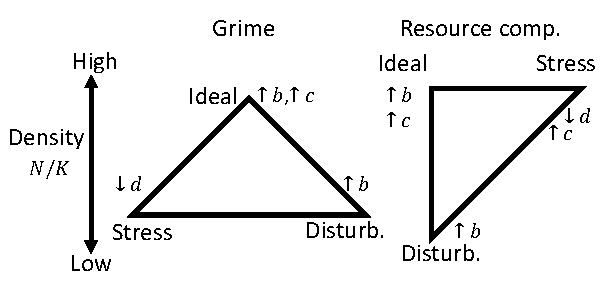
\includegraphics[scale=1]{axes.pdf}
\caption{\label{fig:axes} The realization of Grime's triangle in our model. Schematic representation of the triangular space bounded by the low/high extremes of stress/disturbance. The low-$T$ interpretation of stress is also shown. The vertices of the triangles correspond to different environmental extremes. Selection favors different traits at each vertex, leading to different trait clusters.} 
\end{figure}

%How does Fig.~4 compare to empirical analyses of Grime's C/S/R strategies? In our comparison we will stick to fishes, corals and plants, for which three-way primary strategy schemes are well developed \citep{grime_1977,winemiller_1992,darling_2012}. The connection of our model to fish strategies is necessarily more tentative, given that fishes are motile and not all territorial. 
%
%In disturbed environments, we predict evolution for higher $b$ and lower $d$, but not higher $c$. Higher $b$ means higher fecundity and/or dispersal ability (see ``Model''). This is consistent with a ruderal strategy. Plant ruderals devote a large proportion of their productivity to seed production \citep{grime_1977}, whereas the analogous ``opportunist'' fishes have large intrinsic growth rates \citep{winemiller_1992}. In corals, ruderals are distinguished by brood spawning (rather than broadcast spawning; \citealt{darling_2012}). This corresponds to higher parental investment and lower overall propagule production --- counter-intuitively, a stereotypical ``$K$-selected'', high-density trait \citep{pianka_1970}. However, since broadcast spawners are vulnerable to an Allee effect at the egg fertilization stage \citep{knowlton_2001}, brood spawning could actually be a way to ensure high $b$ at low densities \citep{darling_2012}. Lower $d$ could be achieved by improved individual resistance to physical destruction, but it is hard to reduce mortality in the face of severe disturbances. Alternatively, shortening the time to reproductive maturity (the iteration time in our model) is an effective way of reducing the chance of death per iteration, $d$, for a given frequency of disturbance. An exceptionally short life cycle is probably the most defining characteristic of ruderals \citep{grime_1977,winemiller_1992,darling_2012}. Note that if evolution manages to appreciably reduce $d$ for a given disturbance intensity, then the population no longer lies at the extreme disturbance vertex of Grime's triangle. Thus, ruderals are characterized by both high $b$ and high $d$, but there is a constant pressure for a shorter life cycle, extending the limits of disturbance that can be tolerated. 
%
%In stressful environments, we predict evolution for lower $d$, and also  for higher $c$ in the high-density interpretation of stressful environments. Low $d$ is essential when $b\ll 1$, and stress tolerant plants and corals have long life spans, allowing for long intervals between successful recruitments (and episodic broadcast spawning in corals). For fishes, the ``equilibrium'' strategy is the analogue of Grime's stress tolerator. This strategy is associated with consumable resource limitation, and is also characterized by long life span, as well as high parental investment in tiny broods. This may reflect a high-$c$ strategy in the face of intense competition for severely limited resources (the high-density interpretation).
%
%In ideal environments, we predict evolution for higher $b$ and $c$, but not lower $d$. In plants and corals, a key mechanism for winning territorial contests (higher $c$) is rapidly outgrowing and ``shading out'' competitors; empirically, rapid individual growth is a defining feature of the competitor trait cluster \citep{grime_1977,darling_2012}. The situation for $b$ is more ambiguous. Competitor strategies in plants and corals span a range of $b$. For fishes, the analogous ``periodic'' strategy is characterized by enormous spawn sizes as well as rapid development \citep{winemiller_1992,winemiller_2015}. The role of $b$ in ideal environments will be discussed further below.

\subsection*{Coexistence in constant and cyclical environments}\label{sec:invas}

In the previous section we only considered the how $b$, $c$ and $d$ should respond in Grime's environmental extremes. Here we further explore the low frequency behavior of Eq. \eqref{eq:master} to determine which types can coexist in a constant environment, and then consider the full time-dependent behaviour of Eq. \eqref{eq:master} in a cyclical environment. 

In a population with a single genotype $i$ which is in equilibrium, $R_i=0$, $\overline{c}=c_i$ and $\Delta n_i = 0$, and Eq. \eqref{eq:master} gives
\begin{equation}
b_i\left(e^{-L}+A_i\right)-d_i=0,\label{eq:equil}
\end{equation}
where $A_i=(1-(1+L)e^{-L})/L$. Now suppose that a new genotype $j$, which is initially rare, appears in the population. Then $A_j\ll R_j$, $l_j\approx 0$ and $\overline{c}\approx c_i$, and so, from Eq. \eqref{eq:master}, $n_j$ will increase if 
\begin{equation}
b_j \left(e^{-L}+R_j\frac{c_j}{c_i}\right)-d_j>0,\label{eq:invad}
\end{equation}
where $R_j\approx (1-e^{-L})/\left(\frac{c_j}{c_i}+\frac{L-1-e^{-L}}{1-(1+L)e^{-L}}\right)$. 

Stable coexistence is possible between genotypes that are superior in different traits. Suppose that $j$ is better at securing territories ($c_j>c_i$), that $i$ is better at producing propagules ($b_i>b_j$), and that $d_i=d_j$. Coexistence occurs if $j$ will invade an $i$-dominated population, but $i$ will also invade a $j$-dominated population (``mutual invasion''). If $b_i$ is so large that $L\gg 1$ when $i$ is dominant, and $b_j$ is so small that $L\ll 1$ when $j$ is dominant, then, combining Eqs. \eqref{eq:equil} and \eqref{eq:invad}, we find that $i$ invades $j$ because $b_i>b_j$, while $j$ invades $i$ provided that
\begin{equation}
b_jc_jR_j-b_i c_i A_i>0. \label{eq:jinvadcoex}
\end{equation}
Thus, coexistence occurs if $c_j/c_i$ is large enough. This is a version of the classic competition-colonization trade-off \citep{tilman_94,levins_71}: the competitor ($c$-specialist) leaves many territories unoccupied (low $L$) due to its poor colonization ability (low $b$), which the colonizer ($b$-specialist) can then exploit. A similar argument applies for coexistence between high-$c$ and low-$d$ specialists; a ``competition-longevity'' trade-off \citep{tilman_94}. These forms of co-existence require density dependence, and are not present in the classic lottery model. Mutual invasibility is not possible between $b$- and $d$-specialists. 

Now suppose that birth and death rates vary periodically with amplitude sufficent to cause large changes in population density. This example is inspired by natural \textit{Drosophila} populations, which expand rapidly in the warmer months when fruit is abundant, but largely die off in the colder months. Within this seasonal population density cycle, hundreds of polymorphisms also cycle in frequency \citep{bergland_14}. Some of these polymorphisms may be adaptive and potentially millions of years old, suggesting stable coexistence \citep{bergland_14,messer_2016}. Selection on allele frequencies thus occurs on the same time scale as population demography, a situation vastly more complicated than classical sweeps in demographically stable populations \citep{messer_2016}.

The classical population genetic treatment of fluctuating selection suggests that environmental fluctuations do not promote coexistence. Allele frequencies are successively multiplied by relative fitness values for each environmental iteration, and so two alleles favored in different enviroments can only stably coexist if the product of fitnesses for one type exactly equals the product for the other \citep{dempster_1955}. Thus, stable coexistence still requires frequency-dependent selection or heterozygote advantage (as is required in a constant environment). 

This classical argument overlooks two effects that are present in our extended lottery model. The first is the storage effect, which requires part of the population to be protected from selection each iteration (as occurs when generations are non-overlapping) \citep{chesson_1981}, and which is also present in the classic lottery model. The second is the  bounded population size effect of \cite{yi_2013}, which requires fluctuations in population density and density-dependent regulation of population growth.

%two general mechanisms by which fluctuating selection promotes coexistence. The first is the ``storage effect'', which introduces a form of frequency dependent selection that promotes coexistence in the presence of environmental fluctuations but not in a constant environment. The storage effect occurs when some individuals are protected from selection; in the lottery model a fraction $(1-d_i)n_i$ of each type's adults do not experience selection in a given iteration. Protection from selection promotes coexistence in fluctuating environments because abundant types cannot fully exploit environmental periods that favor them (since only a fraction of the rare type can be displaced), whereas rare types gain the full benefits of their favorable periods (far more adults from the abundant type die than can possibly be replaced by the rare types) \citep{chesson_1981}.

%The second mechanism we will call the ``bounded density effect'', since it is a consequence of the inhibition of reproduction at high population densities (Dempster's (1955) argument ignores density-dependent effects). If there is growth from low to high density in each environmental cycle, then types that are abundant determine the time available for growth every cycle, with less time spent growing in cycles where they are favored, and more in cycles where they are not. This promotes coexistence even in the absence of frequency-dependent selection \citep{yi_2013}. 

Figure \ref{fig:fluctuatingselection} shows the behavior of Eq. \eqref{eq:master} for an example where $b$ and $d$ cycle between zero and positive values (``summers'' with rapid growth and no mortality, and ``winters'' with mortality and no growth). Both the storage effect (adults are sheltered from selection during the summer growth phase) and the bounded density effect (expansion to high density occurs every cycle) are operating. Two types are present, a $b$ specialist, which is better at rapidly growing in the summer (higher $b$), and a $d$ specialist which is better at surviving the winter (lower $d$).  

Neither type has an advantage over a full environmental cycle, and they stably coexist. This is due to some combination of the storage and bounded population size effects (stable coexistence between $b$ and $d$ specialists was not possible in a constant environment). The classic lottery model gives dramatically different co-existence predictions in this scenario (keeping all other parameters the same, the birth rate of the winter survivor must be about $5$ times smaller). This occurs because density returns immediately to capacity $N=T$ in the first summer iteration, after which type frequencies remain constant until the winter. The $d$ specialist thus effectively has infinitely many propagules to secure its winter frequency gains, an enormous advantage compared to the finite propagule density dynamics in Fig. \ref{fig:fluctuatingselection}. Similar difficulties arise in previous models of how the storage effect promotes genetic variation \citep{ellner_1994}, which assume that the total number of offspring per iteration is constant. Beyond this observation, disentangling the storage and bounded population size effects is not straightforward, and requires a more detailed discussion of each effect than we have space for here. Our model is well suited for such a disentangling since it extends the canonical example of the storage effect to allow for density dependent effects.

\begin{figure}
\centering
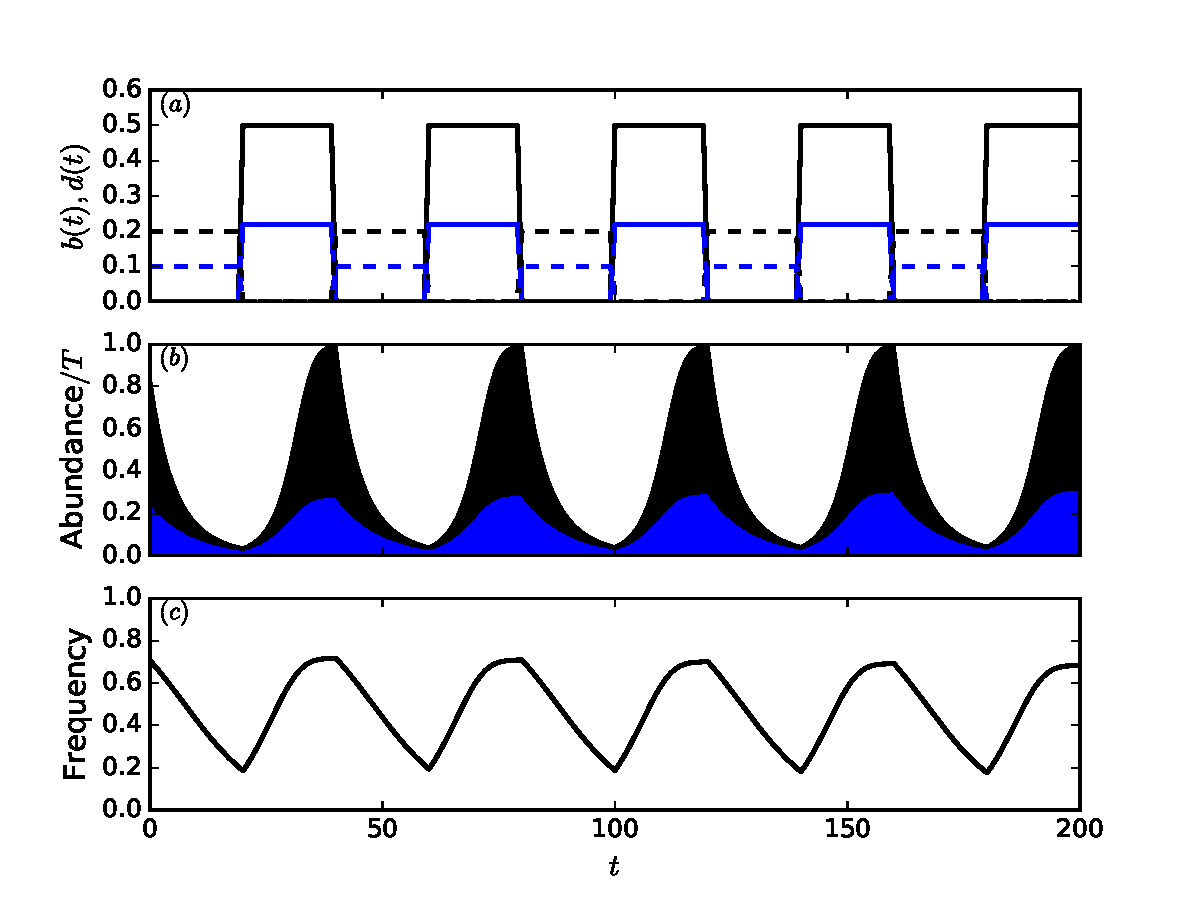
\includegraphics[scale=0.7]{fluctuatingselection.pdf}
\caption{\label{fig:fluctuatingselection} Stable coexistence between $b$ and $d$ specialists in a fluctuating environment. (a) Birth and death rates seasonally alternate being nonzero (white for winter, green for summer). The $b$ specialist (black) has higher $b$ and $d$ ($b=0.5$, $d=0.2$) than the $d$ specialist ($b=0.2$, $d=0.1$) (blue). (b) Both types grow during the positive $b$ phase, and decline during the positive $d$ phase, but the $d$ specialist does so at a lower rate. Total height (blue+black) is population density $N/T$. (c) Summer favors the $b$ specialist, winter the $d$ specialist, and they stably coexist. For illustration, the propagule abundances are assumed to have the form $m_i=b_i(1-N/T)n_i$, reflecting non-directed disperal.} 
\end{figure}

\section*{Discussion}

In the introduction we mentioned the recurring difficulties with confounding selection and demography in population genetic inference. While we have not directly attempted to perform inference with our model, and Eq. \eqref{eq:master} may not be appropriate for particular inference problems, it seems that something similar (and hopefully more analytically tractable) to our extension of the lottery model is unavoidable because, fundamentally, selective births and deaths affect both  abundances and frequencies, not one or the other in isolation. Moreover, some aspects of allele frequency change are intrinsically density dependent. In the classic lottery model, which as we have seen is essentially the Wright-Fisher model with overlapping generations, $b_i$ and $c_i$ are  equivalent in the sense that the number of territorial victories only depends on the product $b_i c_i$ (see ``Model''). This is no longer the case in our extension, where $b$ and $c$ specialists can co-exist. This ``colonization-competition trade-off'' is well known in the co-existence literature \citep{tilman_94}. It and similar forms of ``spatial co-existence'' in stable environments have previously been modeled either with Levin's  qualitative representation of competition \citep{levins_71,tilman_94}, as opposed to the quantitative $c$ of lottery competition, or with a more sophisticated treatment of space (non-uniform dispersal; \citealt{shmida_84,bolker_99}). In cyclical environments, polymorphisms can be stablized by the bounded density effect which is  completely lost if there is an exclusive focus on allele frequencies \citep{yi_2013}. We leave thedetails of how our model might be applied in inference, including the crucial issue of its genetic drift predictions, for future work. 

It is interesting to compare the predictions of the extended lottery model with earlier approaches, such as the $r$/$K$ scheme. While adaptive evolution in the direction predicted by our model does produce traits broadly consistent with Grime's scheme, trait data on selection for higher $b$ at high density was ambiguous. This prediction is also counter to the expectations of MacArthur's $r$/$K$ dichotomy \citep{macarthur_1967}, since $b$ is closely related to the maximal, low-density growth rate $r=b-d$ \citep{pianka_1972}, yet in the $r$/$K$ scheme, high density populations should be subject to $K$, not $r$, selection. Yet it is not surprising that $b$ can matter at high densities. In our model (or any lottery model of competition), $b$ matters at high densities because territorial contests among juveniles are intrinsically unpredictable. This is a realistic feature of the model. Even if one genotype is guaranteed to win a territory in a ``fair'' contest (e.g. it is the most efficient exploiter of a limiting consumable resource; \citealt{tilman_1982}), inferior competitors can win by chance. For example, an inferior competitor's propagules may happen to arrive first, gaining a decisive developmental advantage. First arrivals are more likely to occur for genotypes with a fecundity and/or dispersal advantage, as represented by higher $b$ in lottery models. The analogous intuition in the Wright-Fisher model is that fecundity confers a relative fitness advantage, even though population size is not changing. The logistic model for which $r$ and $K$ are named, does not capture this intuition. 

Confusingly, the term ``$K$-selection'' sometimes refers generally to selection at high density \citep{pianka_1972}, encompassing both selection for higher saturation density \citep{macarthur_1967} and competitive ability \citep{gill_1974}. Contrary to an $r$/$K$ dichotomy, empirical studies have shown that maximal growth rate and saturation density (measured by abundance) are positively correlated, both between species/strains \citep{luckinbill_1979,kuno_1991,hendriks_2005,fitzsimmons_2010}, and as a result of experimental evolution \citep{luckinbill_1978,luckinbill_1979}. From the perspective of our model, this correlation is not surprising since the saturation density, which is determined by a balance between births and deaths, increases with $b$. 

There is support for a negative relationship between competitive success at high density and maximal growth rate \citep{luckinbill_1979}, consistent with an $r$/$K$ dichotomy. This could be driven by a tradeoff between individual size and reproductive rate. To avoid confusion with other forms of ''$K$-selection'', selection for competitive ability has been called ``$\alpha$-selection'' after the competition coefficients in the Lotka-Volterra equation \citep{gill_1974,case_1974,joshi_2001}. However, competitive success as measured by $\alpha$ (i.e. the per-capita effect of one genotype on another genotype's growth rate) is only partly determined by individual competitive ability --- in the presence of age-structured competition and territoriality, it also includes the ability of each genotype to produce contestants i.e. $b$ in our model. Our $c$ is strictly competitive ability only --- as such, changes in $c$ do not directly affect population density (the total number of territories occupied in an iteration is $\Delta_+ N=U(1-e^{-L})$, which does not depend directly on the $c_i$). The clean separation of a strictly-relative $c$ parameter is particularly useful from an evolutionary genetics perspective, essentially embedding a zero-sum relative fitness trait within a non-zero-sum fitness model. This could have interesting applications for modeling the impacts of intra-specific competition on species extinction, for example due to clonal interference \citep{gerrish_1998,desai_2007} between $c$-strategists on the one hand, and $b$- and $d$- strategists on the other.

$K$-selection in the narrow logistic sense of selection for a greater environmental carrying capacity for given birth and death rates, sometimes referred to as ``efficiency'' \citep{macarthur_1967}, could be represented in our model by smaller individual territorial requirements. To a first approximation, two co-occurring genotypes which differ by a small amount in their territorial requirements only should have the same fitness since the costs or benefits of a change in the amount of unocupied territory is shared equally among genotypes via the propagule density per territory $L$. The situation is more complicated when the differences in territorial requirements become large enough that territorial contests can occur on different scales for different genotypes. We leave these complications for future work. 

Our realization of Grime's triangle (Fig.~4) differs from approaches which identify primary strategies as trait combinations which can co-exist \citep{bolker_99}, referring instead to the direction of adaptive trait evolution under different regimes of stress and disturbance, which is closer in spirit to Grime's arguments \citep{grime_1974,grime_1977}. In addition, we have not assumed any kind of trade-offs or pleitropy between $b$, $c$ and $d$, only constraints imposed by the environment on the order of magnitude of $b$ and $d$. As an example of a trade-off, corals which rapidly out-shade neighbors have a tall, branched morphology which is vulnerable to disturbances, and so, all else being equal, ideal environment $c$-strategists will suffer higher mortality from disturbances \citep{darling_2012}. Fig.~\ref{fig:axes} gives the same conclusion without invoking trade-offs; mutations which reduce disturbance vulnerability are essentially neutral under ideal conditions, leading to no improvements in mortality from disturbances, whereas $c$ will tend to increase over time. Thus, while trade-offs may amplify specialization, and are sometimes invoked to explain primary strategy schemes \citep{macarthur_1967,winemiller_1992,aerts_1999}, they are not necessary for it.

One limitation of our model as a general-purpose model of density-dependent selection is the restriction of competition to interference competition between juveniles for durable resources (lottery recruitment to adulthood), analogous to the ubiquitous assumption of viability selection in population genetics \citep[p. 45]{ewens_2004}. In some respects this is the complement of resource competition models, which restrict their attention to exploitation competition, typically without age structure \citep{tilman_1982}. In the particular case that resources are spatially localized (e.g. due to restricted movement through soils), resource competition and territorial acquisition effectively coincide, and in principle resource competition could be represented by a competitive ability $c$ (or conversely, $c$ should be derivable from resource competition). The situation is more complicated if the resources are well-mixed, since, in general, resource levels then need to be explicitly tracked. It seems plausible that explicit resource tracking may not be necessary when the focus is on the evolution of similar genotypes rather than the stable co-existence of widely differing species \citep{ram_2016}. We are not aware of any attempts to delineate conditions under which explicit resource tracking is unnecessary even if it is assumed that community structure is ultimately determined by competition for consumable resources. More work is needed connecting resource competition models to the density-dependent selection literature, since most of the former has to date been focused on narrower issues of the role of competition at low resource availability \citep{aerts_1999,davis_1998,tilman_2007}.  

While our model can be applied to species rather than genotypes (e.g. ecological invasions), our focus is genotype evolution. Our assumption that there are no large $c$ discrepancies (section ``Mean field approximation'') amounts to a restriction on the amount of genetic variation in $c$ in the population. Since beneficial mutation effect sizes will typically not be much larger than a few percent, large $c$ discrepancies can only arise if the mutation rate is extremely large, and so the assumption will not be violated in most cases. However, this restriction could become important when looking at species interactions rather than genotype evolution.

%\section*{Acknowledgments}

%We thank Peter Chesson and Joachim Hermisson for many constructive comments on this manuscript. This work was financially supported by the National Science Foundation (DEB-1348262).

\bibliographystyle{amnatnat}
\bibliography{reference} 

\section*{Appendix A: Poisson approximation}

For simplicity of presentation, we have assumed a Poisson distribution for the $x_i$ as our model of dispersal. Strictly speaking, the total number of $i$ propagules $\sum x_i$ (summed over unoccupied territories) is then no longer a constant $m_i$, but fluctuates between generations for a given mean $m_i$, which is more biologically realistic. Nevertheless, since we do not consider the random fluctuations in type abundances here, and for ease of comparison with the classic lottery model, we ignore the fluctuations in $m_i$. Instead we focus, on Poisson fluctuations in propagule composition in each territory. 

In the exact model of random dispersal, the counts of a genotype's propagules across unnocupied territories follows a multinomial distribution with dimension $U$, total number of trials equal to $m_i$, and equal probabilities $1/U$ for a propagule to land in a given territory. Thus, the $x_i$ in different territories are not independent random variables. However, for sufficiently large $U$ and $m_i$, this multinomial distribution for the $x_i$ across territories is closely approximated by a product of independent Poisson distributions for each territory, each with rate parameter $l_i$ \citep[Theorem 1]{arenbaev_1977}. Since we are ignoring finite population size effects, we effectively have $T\rightarrow \infty$, in which case $U$ can be only be small enough to violate the Poisson approximation if there is vanishing population turnover, and then the dispersal distribution is irrelevant anyway. Likewise, in ignoring stochastic finite population size for the $n_i$, we have effectively already assumed that $m_i$ is large enough to justify the Poisson approximation (the error scales as $1/\sqrt{m_i}$; \citealt{arenbaev_1977}).

\section*{Appendix B: Derivation of growth equation}

We separate the right hand side of Eq.~\eqref{eq:growthsumuncoupled} into three components $\Delta_+ n_i = \Delta_u n_i+\Delta_r n_i+\Delta_a n_i$ which vary in relative magnitude depending on the propagule densities $l_i$. Following the notation in the main text, the Poisson distributions for the $x_i$ (or some subset of the $x_i$) will be denoted $p$, and we use $P$ as a general shorthand for the probability of particular outcomes.

\subsection*{Growth without competition}

The first component, $\Delta_u n_i$, accounts for territories where only one focal propagule is present $x_i=1$ and $x_j=0$ for $j\neq i$ ($u$ stands for ``uncontested''). The proportion of territories where this occurs is $l_i e^{-L}$, and so 
\begin{equation}
\Delta_u n_i=Ul_i e^{-L}=m_i e^{-L}.
\end{equation}

\subsection*{Competition when rare}

The second component, $\Delta_r n_i$, accounts for territories where a single focal propagule is present along with at least one non-focal propagule ($r$ stands for ``rare'') i.e. $x_i=1$ and $X_i\geq 1$ where $X_i=\sum_{j\neq i} x_j$ is the number of nonfocal propagules. The number of territories where this occurs is $Up_i(1)P(X_i\geq 1)=b_i n_i e^{-l_i}(1-e^{-(L-l_i)})$. Thus 
\begin{equation}
\Delta_r n_i = m_i e^{-l_i}(1-e^{-(L-l_i)})\left\langle  \frac{c_i}{c_i +\sum_{j\neq i} c_j x_j } \right\rangle_{\tilde{p}},  \label{eq:deltr}
\end{equation}
where $\langle \rangle_{\tilde{p}}$ denotes the expectation with respect to $\tilde{p}$, and $\tilde{p}$ is the probability distribution of nonfocal propagule abundances $x_j$ \textit{after} dispersal, in those territories where exactly one focal propagule, and at least one non-focal propagule, landed. 

Our ``mean field'' approximation is to replace $x_j$ with its mean in the last term in Eq.~\eqref{eq:deltr},
\begin{equation}
\left\langle\frac{c_i}{c_i +\sum_{j\neq i} c_j x_j}\right\rangle_{\tilde{p}}\approx \frac{c_i}{c_i +\sum_{j\neq i} c_j \langle x_j\rangle_{\tilde{p}}}.\label{eq:meanfieldr}
\end{equation}
Below we justify this replacement by arguing that the standard deviation $\sigma_{\tilde{p}}(\sum_{j\neq i} c_j x_j)$ (with respect to $\tilde{p}$), is much smaller than $\langle\sum_{j\neq i} c_j x_j\rangle_{\tilde{p}}$.

We first calculate $\langle x_j \rangle_{\tilde{p}}$. Let $X=\sum_j x_j$ denote the total number of propagules in a territory and ${\mathbf x_i}=(x_1,\ldots,x_{i-1},x_{i+1}\ldots,x_G)$ denote the vector of non-focal abundances, so that $p({\mathbf x_i})=p_1(x_1)\ldots p_{i-1}(x_{i-1})p_{i+1}(x_{i+1})\ldots p_G(x_G)$. Then, $\tilde{p}$ can be written as
\begin{align}
\tilde{p}({\mathbf x_i})&=p({\mathbf x_i}|X\geq 2,x_i=1)\nonumber\\
&=\frac{P({\mathbf x_i},X\geq 2|x_i=1)}{P(X\geq 2)}\nonumber\\
&=\frac{1}{1-(1+L)e^{-L}}\sum_{X=2}^{\infty} P(X) p({\mathbf x_i}|X_i=X-1),
\end{align}
and so
\begin{align}
\langle x_j \rangle_{\tilde{p}}&=\sum_{\mathbf x_i} \tilde{p}({\mathbf x_i})x_j\nonumber\\
&=\frac{1}{1-(1+L)e^{-L}}\sum_{X=2}^{\infty} P(X) \sum_{\mathbf x_i} p({\mathbf x_i}|X_i=X-1)x_j.
\label{eq:raremonster1}
\end{align}
The inner sum over ${\mathbf x_i}$ is the mean number of propagules of a given nonfocal type $j$ that will be found in a territory which received $X-1$ nonfocal propagules in total, which is equal to $\frac{l_j}{L-l_i}(X-1)$. Thus, 
\begin{align}
\langle x_j \rangle_{\tilde{p}}&=\frac{l_j}{1-(1+L)e^{-L}}\frac{1}{L-l_i}\sum_{k=2}^{\infty} P(X) (X-1)\nonumber\\
&=\frac{l_j}{1-(1+L)e^{-L}}\frac{L-1+e^{-L}}{L-l_i},
\label{eq:meanxjrare}
\end{align}
where the last line follows from $\sum_{X=2}^{\infty} P(X)(X-1)=\sum_{X=1}^{\infty} P(X)(X-1)=\sum_{X=1}^{\infty} P(X)X-\sum_{X=1}^{\infty}P(X)$.

The exact analysis of the fluctuations in $\sum_{j\neq i} c_j x_j$ is complicated because the $x_j$ are not independent with respect to $\tilde{p}$. These fluctuations are part of the ``drift'' in type abundances which we leave for future work. Here we use the following approximation to give some insight into the magnitude of these fluctuations and also the nature of the correlations between the $x_j$. We replace $\tilde{p}$ with $\tilde{q}$, defined as the ${\mathbf x_i}$ Poisson dispersal probabilities conditional on $X_i\geq1$ (which are independent). The distinction between $\tilde{p}$ with $\tilde{q}$ will be discussed further below. The $\tilde{q}$ approximation gives $\langle x_j \rangle_{\tilde{q}}=\langle x_j \rangle_p/C=l_j/C$, 
\begin{align}
\sigma_{\tilde{q}}^2(x_j)&=\langle x_j^2 \rangle_{\tilde{q}}-\langle x_j \rangle_{\tilde{q}}^2\nonumber\\
&=\frac{1}{C}\langle x_j^2 \rangle_p-\frac{l_j^2}{C^2}\nonumber \\
&=\frac{1}{C}(l_j^2 + l_j)-\frac{l_j^2}{C^2}\nonumber \\
&=\frac{l_j^2}{C}\left(1-\frac{1}{C}\right)+\frac{l_j}{C},\label{eq:varr}
\end{align}
and 
\begin{align}
\sigma_{\tilde{q}}(x_j,x_k)&=\langle x_j x_k \rangle_{\tilde{q}}-\langle x_j \rangle_{\tilde{q}}\langle x_k \rangle_{\tilde{q}}\nonumber\\
&=\frac{1}{C}\langle x_j x_k \rangle_p-\frac{l_jl_k}{C^2}\nonumber\\
&=\frac{l_j l_k}{C}\left(1-\frac{1}{C}\right),\label{eq:covr}
\end{align}
where $C=1-e^{-(L-l_i)}$ and $j\neq k$. 

The exact distribution $\tilde{p}$ assumes that exactly one of the  propagules present in a given site after dispersal belongs to the focal type, whereas $\tilde{q}$ assumes that there is a focal propagule present before non-focal dispersal commences. As a result, $\tilde{q}$ predicts that the mean propagule density is greater than $L$ (in sites with only one focal propagule is present) when the focal type is rare and the propagule density is high. This is erroneous, because the mean number of propagules in every site is $L$ by definition. Specifically, if $L-l_i \approx L\gg 1$, then the mean propagule density predicted by $\tilde{q}$ is approximately $L+1$. The discrepancy causes rare invaders to have an intrinsic rarity disadvantage (territorial contests under $\tilde{q}$ are more intense than they should be). In contrast, Eq. \eqref{eq:meanxjrare} correctly predicts that there are on average $\sum_{j\neq i}\langle x_j \rangle_{\tilde{p}}\approx L-1$ nonfocal propagules because $\tilde{p}$ accounts for potentially large negative covariances between the $x_j$ ``after dispersal''. By neglecting the latter covariences, $\tilde{q}$ overestimates the fluctuations in $\sum_{j\neq i} c_j x_j$; thus $\tilde{q}$ gives an upper bound on the fluctuations. The discrepancy between $\tilde{q}$ and $\tilde{p}$ will be largest when $L$ is of order $1$ or smaller, because then the propagule assumed to already be present under $\tilde{q}$ is comparable to, or greater than, the entire propgaule density. 

Decomposing the variance in $\sum_{j\neq i} c_j x_j$,
\begin{equation}
\sigma_{\tilde{q}}^2(\sum_{j\neq i} c_j x_j)=\sum_{j\neq i}\left[c_j^2\sigma_{\tilde{q}}^2(x_j)+2\sum_{k>j, k\neq i}c_j c_k\sigma_{\tilde{q}}(x_j,x_k)\right],\label{eq:vartotr}
\end{equation}
and using the fact that $\sigma_{\tilde{q}}(x_j,x_k)$ and the first term in Eq. \eqref{eq:varr} are negative because $C<1$, we obtain an upper bound on the relative fluctuations in $\sum_{j\neq i} c_j x_j$, 
\begin{equation}
\frac{\sigma(\sum_{j\neq i} c_j x_j)}{\langle\sum_{j\neq i} c_j x_j\rangle}=C^{1/2}\frac{\left(\sum_{j\neq i}c_j^2 l_j+(1-1/C)\left(\sum_{j\neq i}c_j l_j\right)^2 \right)^{1/2}}{\sum_{j\neq i}c_j l_j}<C^{1/2}\frac{\left(\sum_{j\neq i}c_j^2 l_j\right)^{1/2}}{\sum_{j\neq i}c_j l_j}. \label{eq:cvr}
\end{equation}

Suppose that the $c_j$ are all of similar magnitude (their ratios are of order one). Then Eq.~\eqref{eq:cvr} is $\ll 1$ for the case when $L-l_i \ll 1$ (due to the factor of $C^{1/2}$), and also for the case when at least some of the nonfocal propagule densities are large $l_j\gg 1$ (since it is then of order $1/\sqrt{L-l_i}$). The worst case scenario occurs when $L-l_i$ is of order one. Then Eq.~\eqref{eq:cvr} gives a relative error of approximately $50\%$, which from our earlier discussion we know to be a substantial overestimate when $L$ is of order $1$. Our numerical results (Fig. \ref{fig:simcomp}) confirm that the relative errors are indeed small.

However, the relative fluctuations in $\sum_{j\neq i} c_j x_j$ can be large if some of the $c_j$ are much larger than the others. Specifically, in the presence of a rare, extremely strong competitor ($c_j l_j\gg c_{j'} l_{j'}$ for all other nonfocal genotypes $j'$, and $l_j\ll 1$), then the RHS of Eq. \eqref{eq:cvr} can be large and we cannot make the replacement Eq.~\eqref{eq:meanfieldr}. 

Substituting Eqs. \eqref{eq:meanfieldr} and \eqref{eq:meanxjrare} into Eq.~\eqref{eq:deltr}, we obtain
\begin{equation}
\Delta_r n_i\approx m_i R_i\frac{c_i}{\overline{c}}, \label{eq:deltrfinal}
\end{equation}
where $R_i$ is defined in Eq.~\eqref{eq:Dr}.

\subsection*{Competition when abundant}

The final contribution, $\Delta_a n_i$, accounts for territories where two or more focal propagules are present ($a$ stands for ``abundant"). Similarly to Eq.~\eqref{eq:deltr}, we have 
\begin{equation}
\Delta_a n_i=U(1-(1+l_i)e^{l_i})\left\langle \frac{c_i x_i}{\sum_j c_j x_j} \right\rangle_{\hat{p}}\label{eq:delta}
\end{equation}
where $\hat{p}$ is the probability distribution of both focal and nonfocal propagaule abundances \textit{after} dispersal in those territories where at least two focal propagules landed. 

Again, we argue that the relative fluctuations in $\sum c_j x_j$ are much smaller than $1$ (with respect to $\hat{p}$), so that,
\begin{equation}
\left\langle \frac{c_i x_i}{\sum_j c_j x_j} \right\rangle_{\hat{p}}\approx  \frac{c_i \langle x_i \rangle_{\hat{p}}}{\sum_j c_j \langle x_j\rangle_{\hat{p}}}.\label{eq:meanfielda}
\end{equation}
Following a similar procedure as for $\Delta_r n_i$, where the vector of propagule abundances is denoted ${\mathbf x}$, the mean focal genotype abundance is, 
\begin{align}
\langle x_i \rangle_{\hat{p}}&=\sum_{\mathbf x} x_i p(\mathbf x|x_i\geq 2)\nonumber \\
&=\sum_{x_i} x_i p(x_i|x_i\geq 2) \nonumber\\
&=\frac{1}{1-(1+l_i)e^{-l_i}}\sum_{x_i\geq 2} p(x_i)x_i\nonumber\\
&=l_i\frac{1-e^{-l_i}}{1-(1+l_i)e^{-l_i}}.
\end{align}
For nonfocal genotypes $j\neq i$, we have
\begin{align}
\langle x_j \rangle_{\hat{p}}&=\sum_{\mathbf x} x_j p(\mathbf x|x_i\geq 2)\nonumber \\
&=\sum_{X}P(X|x_i\geq 2)\sum_{\mathbf x} x_j p({\mathbf x}|x_i\geq 2,X)\nonumber\\
&=\sum_{X}P(X|x_i\geq 2)\sum_{x_i} p(x_i|x_i\geq 2,X) \sum_{\mathbf x_i} x_j p(\mathbf x_i|X_i=X-x_i)\nonumber\\
&=\sum_{X}P(X|x_i\geq 2)\sum_{x_i}p(x_i|x_i\geq 2,X) \frac{l_j(X-x_i)}{L-l_i} \nonumber\\
&=\frac{l_j}{L-l_i}\left[\sum_{X}P(X|x_i\geq 2)X - \sum_{x_i}p(x_i|x_i\geq 2) x_i \right]\nonumber\\
&=\frac{l_j}{L-l_i}\left( L\frac{1-e^{-L}}{1-(1+L)e^{-L}}- l_i\frac{1-e^{-l_i}}{1-(1+l_i)e^{-l_i}}\right). 
\end{align}

To calculate the relative fluctuations in $\sum_{j\neq i} c_j x_j$, we use a similar approximation as for $\Delta_r n_i$: $\hat{p}$ is approximated by $\hat{q}$, defined as the ${\mathbf x}$ dispersal probabilities in a territory conditional on $x_i>2$ (that is, treating the $x_j$ as indepenent). All covariances between nonfocal genotypes are now zero, so that $\sigma_{\hat{q}}^2(\sum c_j x_j)=\sum c_j^2 \sigma_{\hat{q}}^2(x_j)$, where $\sigma_{\hat{q}}^2(x_j)=l_j$ for $j\neq i$, and  
\begin{equation}
\sigma_{\hat{q}}^2(x_i)=\frac{l_i}{D}\left(l_i+1-e^{-l_i}-\frac{l_i}{D}\left(1-e^{-l_i}\right)^2\right),
\end{equation}
where $D= 1-(1+l_i)e^{-l_i}$, and 
\begin{equation}
\frac{\sigma_{\hat{q}}(\sum c_j x_j)}{\langle\sum c_j x_j\rangle} = \frac{\left(\sum_{j\neq i} c_j^2 l_j + c_i^2 \sigma_{\hat{q}}^2(x_i)\right)^{1/2}}{\sum_{j\neq i} c_j l_j + c_i l_i (1-e^{-l_i})/D} \label{eq:cva}.
\end{equation}

Similarly to Eq.~\eqref{eq:cvr}, the RHS of Eq. \eqref{eq:cva} is $\ll 1$ for the case that $L \ll 1$ (due to a factor of $D^{1/2}$), and also for the case when at least some of the propagule densities (focal or nonfocal) are large --- provided that $c_i$ and the $c_j$ are all of similar magnitude. Again, the worst case scenario occurs when $l_i$ and $L-l_i$ are of order $1$, in which case Eq. \eqref{eq:cva} is around $35\%$, which is again where the $\hat{q}$ approximation produces the biggest overestimate of the fluctuations in ${\mathbf x}$. Similarly to Eq.~\eqref{eq:cvr}, the RHS of \eqref{eq:cva} will not be $\ll 1$ in the presence of a rare, extremely strong competitor.  

Combining Eqs. \eqref{eq:delta} and \eqref{eq:meanfielda}, we obtain
\begin{equation}
\Delta_a n_i=m_i A_i \frac{c_i}{\overline{c}},
\end{equation}
where $A_i$ is defined in Eq.~\eqref{eq:Da}.

%\subsection{Logistic growth and classic nesting sites model}

%In the nesting sites model, it is assumed that propagules landing on occupied territory do not survive, while those landing on unoccupied territory immediately occupy the territory. Thus, the probability that a propagule survives is simply $(1-N/K)$, where $N=\sum_i n_i$ is the total population size. Consequently, $n_i$ increases by $1$ over the interval $[t,t+\Delta t]$ with probability $b_i n_i (1-N/K)\Delta t$. Provided that the abundances $n_i$ are large enough that demographic stochasticity is negligible (i.e. they have established), we can treat $n_i(t)$ as a continuous variable with growth given by the expectation of $b_i n_i (1-N/K)\Delta t$, and so, taking $\Delta t \rightarrow 0$ we obtain
%\begin{equation}
%\frac{dn_i}{dt}=b_i\left(1-\frac{N}{K}\right)n_i. \label{eq:logistic}
%\end{equation}

%\section{Territorial availability}
%
%In Sec. \ref{sec:c} we assumed that adults have the same territorial requirement, regardless of genotype. This can be generalized to allow genotypes to differ in their territorial requirements. Each adult from genotype $i$ now requires $t_i$ units of territory, $T$ is the total territory available to the population, and $T-\sum_i t_i$ units of territory are unoccupied. 
%
%Competition between propagules with different territorial requirements is potentially much more complicated than the model in Sec. \ref{sec:c}, because competition is no longer neatly partitioned into a set of identical territories.  The larger a propagule's territorial requirement, the more neighboring propagules it will interact with during its development to adulthood. 
%
%
%A simple way to avoid these complications is to partition the unoccupied territory into uniform units of territory with size given by the largest territorial requirement $t^*={\rm max}_i t_i$. The uniform territory approach used in Sec.  \ref{sec:c}
%
%The biological intuition behind this 
%
%Thus $U=(T-\sum_i t_i n_i)/t^*$.


\end{document}
